\documentclass{article}
\usepackage[nonatbib]{nips_2016}

\usepackage[breaklinks=true,letterpaper=true,colorlinks,citecolor=black,bookmarks=false]{hyperref}

\usepackage{amsthm}
\usepackage{amsmath,amssymb}
\usepackage{enumitem}

\usepackage[sort&compress,numbers]{natbib}
\usepackage[normalem]{ulem}
\usepackage{subcaption}
% use Times
\usepackage{times}
% For figures
\usepackage{graphicx} % more modern
%\usepackage{epsfig} % less modern
%\usepackage{subfig} 

\graphicspath{{../../figs/}}

\usepackage{chronosys}

\usepackage{tikz}
\usepackage{tkz-tab}
\usepackage{caption} 
\usepackage{subcaption} 
\usetikzlibrary{shapes.geometric, arrows}
\tikzstyle{arrow} = [very thick,->,>=stealth]

\usepackage{cleveref}
\usepackage{setspace}
\usepackage{wrapfig}
%\usepackage[ruled]{algorithm}
\usepackage{algpseudocode}
\usepackage[noend,linesnumbered]{algorithm2e}

\usepackage[disable]{todonotes}


\title{Machine Learning for Condition Monitoring}

\author{
	Johnathan DiMatteo \\
	School of Computer Science\\
	University of Waterloo\\
	Waterloo, ON, N2L 3G1 \\
	\texttt{jdimatteo@uwaterloo.ca} \\
}

\begin{document}
\maketitle

\begin{abstract} 
\begin{center}
\section*{Abstract}
It remains critical for several important industries to have knowledge of asset health.
A \textit{Condition Monitoring} strategy using machine learning is proposed as a research project for CS 680.
An algorithm will be developed and evaluated on several large scale reheat furnace fans provided by a steel manufacturer.
\end{center}

\end{abstract} 

% who what where when
\section*{Motivation}

An often overlooked part of an asset's expenses is maintenance.
A popular maintenance strategy is known as Preventative Maintenance (PvM), 
where maintenance is regularly performed on an asset while it is still in good condition to prevent it from breaking down unexpectedely.
Over \$ 200 billion is spent on such maintenance every year in the United States and one-third is wasted on improper or unnecessary maintenance \cite{mobley2002introduction}.
Even worse, no maintenance at all can lead to unexpected failures which in turn can cause serious economic consquences or injury.
There exists a significant need to modernize maintenance techniques around the world to ensure safety, reliability, and efficiency.

During the Second World War, a British scientist named Conrad Waddington made a fascinating discovery about the maintenance of aircraft while working for the Royal Air Force (RAF).
Previously, aircraft bombers had a notorious problem of breaking down - in fact the ideal serviceabitity in a squadron of bombers was only around 70-75\% \cite{Morse1364}.
What he discovered was that preventative maintenance methods actually increased the rate of unexpected failure.
The process of more maintenance leading to more failures became known as the Waddington Effect as a result.
By increasing the interval between maintenance cycles and eliminating all maintenance deemed unnecessary,
Waddington was able to increase the effective flight hours of the RAF bomber fleet by 60\% \cite{Morse1364}.

After this discovery, asset owners around the world tried to find the optimal time to repair an asset.
This led to the invention of Predictive Maintenance (PdM), a philosphy that uses the actual operating condition of assets to optimize operations \cite{mobley2002introduction}.
For PdM to be effective, the asset's operating condition must be estimated.
Estimating the asset's operating condition is the focus of the paper, which is refered to as the \textit{health score}.
\section{Background} % Numbered section

%------------------------------------------------
\subsection{Why Machine Learning?}
% why ML?
One of the most common reasons PdM methods fail is a lack of continuous improvement and a lack of repeatability \cite{whypdmfails}.
Additionally, equipment monitoring is a time consuming process, requires experts to identify failure patterns, and is expensive.
Machine learning provides an automated approach that requires minimal asset knowledge, is inexpensive, can be trained on many assets, and can be re-trained as operating conditions change.

Machine learning techniques for predictive maintenance were considered not practical, too complex, or too time consuming.
In particular, plant managers did not want to change their existing infrastructure (the software that handles data acquisition and analyzes it) to adopt the technology.
But now Asset Performance Management (APM) software providers are growing and condition based maintenance is at the forefront.
As they team up with cloud based data solutions, it becomes easy for asset operators to implement machine learning in their existing data infrastructures via a simple call to the cloud.
Manufacturers around the world use APM technology from Bentley Systems, a global leader in APM capabilities according to a recent Gartner report \cite{foust_steenstrup_2018}.
The proposed solution will be deployed and maintained using APM software from Bentley Systems.

\subsection{ArcelorMittal Dofasco}
%\subsection{Steel Manufacturing}
% Who is dofasco
ArcelorMittal Dofasco is a steel company located in Hamilton, Ontario.
They use Bentley's APM software and are eager for a machine learning solution to detect the operating conditions of various assets. 
In particular, they have offered a real data set of several industrial level furnace fans located in the Hamilton plant. 
Specifically, the data is composed of several smaller data sets, each representing various hours of operation.
%See the Appendix for full list of variables included.
% Steel mill 
In a steel making plant, called a steel mill, operations run almost 24/7 except when the mill is shut down once a month for repairs and maintenance.
A failure of an asset leading to a shutdown at any other time results in severe costs.
If the operating condition of the asset is known, then operators can determine whether or not it should not be repaired during that scheduled downtime,
thus avoiding costly unexpected failures and the Waddington Effect.


%What is a reheating furnace?
One of the most costly failures occurs when the fans for the reheating furnace fail.
A reheating furnace is used to raise the internal temperature of steel, so that it can be shaped into a final product.
Setting the correct temperature is one of the most essential factors of product quality in the plant.
In fact, the temperature is so high that if the furnace must be inspected, the entire line must be shut down for days to allow the furnace to cool.
%A subject matter expert from ArcelorMittal suggests this could cost millions of dollars in lost production.
A subject matter expert from the steel manufacturer suggests this could cost millions of dollars in lost production.

% about the failure
%One way these furnaces fail is via a failure of the exhaust fans.

%It is therefore critical to steel manufacturers to replace the exhaust fans before a failure occurs.

%------------------------------------------------

\subsection{Self Organizing Maps}

A Self-Organizing Map (SOM) is a type of neural network that is often used as a dimensionality reduction technique as it produces a low dimensional representation of the training samples \cite{kohonen1997exploration}.
A SOM consists of a number of neurons, each represented by a weight vector. 
They are different from other neural networks because they employ competitive learning.
The basic idea behind competitive learning is to have the neurons compete with each other to see who is the most similar to the input vector, `winner takes all' style.
The similarity is usually defined as the Euclidean distance (Eq. \ref{eq:1}) between the input vector and the weight vectors of each neuron.
\begin{equation} \label{eq:1}
    \Vert \boldsymbol{x - w} \Vert_2
\end{equation}

To create a SOM, the size of the map is set to be approximately $5*\sqrt{n}$, where n is number of data points \cite{Tian2014AnomalyDU}. 
The input data is normalized for each variable and the number of neurons are set.
The weights of the closest neurons are updated for each instance in the input data.
Once training is complete, the SOM can be used again to measure the similarity between a test point and the learned mapping.


\begin{figure}[!h]
    \centering
    \includegraphics[scale=0.5]{som-learning}
    \caption{A SOM mapping the training data to a two dimensional grid.}
    \label{fig:som-learning}
\end{figure}
 
\section{Previous Work}

Using machine learning for condition monitoring is not new.
There are typically three approaches:
\begin{enumerate}
	\item Supervised algorithms using sensor data and maintenance data.
    \item Unsupervised algorithms using only sensor data.
    \item Semi-supervised algorithms using only \textit{healthy} sensor data.
\end{enumerate}

% supervised
Supervised methods require labelled data.
Labelling is the process of associating an output with a set of variable values at a certain point in time.
For example, if there is knowledge to when the failures occurred and there are sufficient failures, the data can be labelled as healthy or not.
Unfortunately, there is just not enough failure data in practice to make this feasible.
Failure data can be estimated and artificially generated but even then the algorithms are limited to a binary outputs \cite{Sotiris2010AnomalyDT}.

Using $k$-nearest neighbours (kNN) to estimate asset condition directly is difficult due to noise, and requires domain specific knowledge to choose appropriate variables.
One paper improves on kNN methods for detecting the levels of severity for cracks in gears \cite{lei2009gear}.
The disadvantage in these approaches is that it requires significant data in a variety of conditions, and it uses classification to identify a severity level instead of a numerical value.

Researchers in \cite{opt} train an autoencoder on healthy imaging data to get a feature representation in a smaller number of dimensions.
Utilizing the Support Vector Machine (SVM), they learn a decision boundary to identify anomalies.
This approach is interesting for high dimensional data but focuses on point anomalies, where as we are interested in projecting asset health over time.

% self organized maps
SOMs have been used in condition maintenance as visualization tools for aircraft engines and ball bearings \cite{come2010aircraft}.
By mapping the input data to a two dimensional grid researchers can identify failures trends.
%Training a SOM on healthy asset data, researchers were able to output a health indication in an interpretable way but still lacked a quantifiable measure \cite{5524339}.
Alternatively, Huang et al. were able to use the minimum quantization error (Eq. \ref{eq:q}) between a test point and the closest neuron of the SOM as the health indicator for ball bearings \cite{som-1}.
% Math equation/formula
\begin{equation}\label{eq:q}
	Q = \min_{k} \Vert D-B_k \Vert
\end{equation}
Where $Q$ is the minimum quantization error, $D$ is a test set observation, and $B_k$ is the weight vector of the $k^{th}$ closest neuron of the SOM.
But, using quantization error can be improved as it is sensitive to noise.
Researchers Tian et al. use a SOM and a $k$-nearest neighbours algorithm in combination with the Euclidean distance between the test data and the healthy data to develop a more robust health score \cite{Tian2014AnomalyDU}.

   
\section{Proposed Work}
\subsection{Implementation}

% unsupervised anomaly score
The project will solve PdM hurdles for operators in modernized workplaces by providing an accurate estimate of asset health.
The proposed method is to replicate the results achieved by other papers using SOMs for condition monitoring. 
Specifically, to train a SOM and get a health score by calculating how much a test data point deviates from normal operation.
The higher the health score, the lower the operating condition of the asset.
Various SOM implementations will be examined, such as the \href{https://pypi.org/project/kohonen/}{Kohonen 1.1.2 Python package} (documentation for this package is sparse).
If these do not provide enough customization then a SOM will be self-coded using Tensorflow.
Customization may be required to allow the comparison of various distance metrics to get a health score.
As discussed, this has been done before but is rarely seen in industry today and the use of these algorithms on real and significant data is challenging and relevant.
For example, the data will be provided in hourly chunks throughout the year (instead of one continuous data set).
Furthermore, pre and post processing techniques will be explored to improve performance, use-ability and interpretability.
Decision boundaries will be learned as a final step (if we have enough failure data) to organize failures into different classes and severity levels.

\begin{figure}[!h]
    \includegraphics[width=3cm]{steps}
    \centering
    \label{fig:steps}
    \caption{Implementation steps from Data.}
\end{figure}

\subsection{Evaluation}

An expected significant challenge will be the model's ability to generalize, given that the data sets span only a days worth of operation in total.
To avoid over-fitting, the number of dimensions will be kept low and regularization will be used where possible.
To judge the models ability to generalize and to evaluate performance, the algorithm will be tested on two data sets: unhealthy operation (1) and healthy operation (2).
Precision was chosen as a metric for (2) to minimize the number of false positives.
This is especially important because this is an experimental project with the steel manufacturer, so it is important that the algorithm does not do more harm than good.
For (1), the algorithm should produce a value indicative of failure at least 75\% of the time.


Performance evaluation of the algorithm from a PdM context will be performed against each of these three scenarios.
\begin{enumerate}
    \item Run-to-Failure: how will the proposed solution compare if no maintenance is performed?
    \item Preventative: how will the proposed solution compare if PvM is performed (the current process of the plant)?
    \item Other Predictive Methods: how will the proposed solution compare if another PdM solution is performed?
\end{enumerate}

Other metrics for evaluation will include the following: cost, latency (time between failure and an indication of failure from the algorithm) and training time.
Finally, the algorithm will also be scrutinized by a subject matter expert (SME) in terms of usability and interpretability.


\subsection{Timeline}

The time from the proposal submission date and the final due date is six weeks.

\begin{enumerate}
	\item Week 1: Choose a SOM algorithm or develop one.
    \item Week 2: Choose a SOM algorithm or develop one.
    \item Week 3: Test algorithm on data, visualize.
    \item Week 4: Choose and evaluate various distance metrics.
    \item Week 5: Tune model, test, repeat. Try pre-processing methods.
    \item Week 6: Report writing and final touch-ups.
\end{enumerate}
\section{Validation and Application}

\subsection{Setup}


\begin{figure}
    \centering
    \resizebox{\linewidth}{!}{% Resize table to fit within
    
    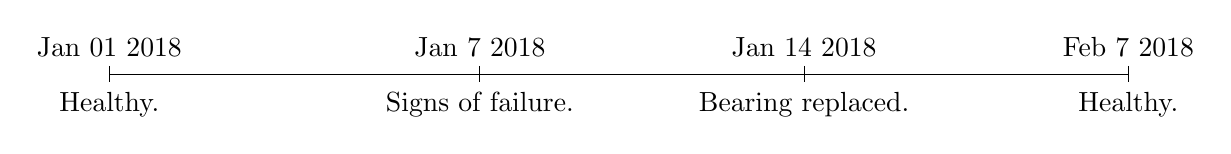
\begin{tikzpicture}[]
    %draw horizontal line
    \draw (0,0) -- (22/1.7,0);
    %draw vertical lines
    \foreach \x in {0, 8, 15, 22}{
       \draw (\x/1.7,3pt) -- (\x/1.7,-3pt);
    }
    %draw nodes
    \draw (0,0) node[below=3pt] { Healthy. } node[above=3pt] { Jan 01 2018  };
    \draw (8/1.7,0) node[below=3pt] { Signs of failure. } node[above=3pt] { Jan 7 2018  };
    \draw (15/1.7,0) node[below=3pt] { Bearing replaced. } node[above=3pt] { Jan 14 2018  };
    \draw (22/1.7,0) node[below=3pt] { Healthy. } node[above=3pt] { Feb 7 2018  };
    \end{tikzpicture}
    }
    \caption{Time Line}
    \label{fig:time_line}
\end{figure}

Four data sets were received representing two weeks, one week, the day of, 
and three weeks after a bearing failure occurred \ref{fig:time_line}.
Each data set has data sampled at an interval of 0.2 milliseconds, although data values are only updated every two milliseconds or so.
After talking to a subject matter expert, it was determined that the data one week and the day of should be considered as failing.
The data two weeks before and three weeks after represent healthy data.
Therefore the experiment setup is as follows:
\begin{enumerate}
    \item the SOM will be trained on data from February 7th.
    \item validation on January 1st data should not show signs of failure, otherwise the model failed to generalize.
    \item evaluation on January 7th and 14th should show signs of failure.
\end{enumerate}


%\begin{figure}
%    \centering
%    \includegraphics[scale=0.5]{som-struct}
%\end{figure}

% describe SOM map
The size of the map was set to be 64, representing a 2D grid 8 by 8 grid of neurons.
Figure \ref{fig:colourmap} shows the SOM after training the map on data from February 7th, where each square represents a neuron. 
The colour indicates how similar neighbouring neurons are, and the number of times a neuron has won a competition is labelled on each neuron.
Neurons with less than two wins are determined to be too noisy for use in the evaluation \cite{som-1}.
These neurons are ignored.
To calculate the health score, the minimum quantization error is averaged over the three closest neurons.
This is analogous to the 3-NN method used by \cite{Tian2014AnomalyDU}.
% this should be explained in detail in previous section but numbers shown here

\begin{figure}[!h]
    \centering
    \includegraphics[width = 0.5\linewidth]{som-colour-map}
    \caption{SOM colour map showing the number of hits for each neuron in the map on the training data.}
    \label{fig:colourmap}
\end{figure}

\subsection{Results}

Operators currently analyze the vibration signals manually.
A vibration expert spends time looking at the raw vibration signals to determine a threshold.
If the threshold is crossed, an alarm is generated.
Operators must manually determine when to replace the bearing based the percentage of time spent above the threshold.
This is a common technique used in a multitude of industries.
The moving average or the standard deviation of the raw signal can also be used.
This method is compared with the SOM and the results are summarized in Table \ref{tbl:percent}.
For all methods the threshold was optimized to get the best results.
Another significant metric to compare the practicality of all methods is the number of alarms generated (see Table \ref{tbl:alarms}).
Ideally, an alarm should trigger only once to indicate failure.

The results of the health score are shown in Figure \ref{fig:health}.
The health score given by the SOM was significantly higher when operators said the bearing was failing.
Upon examination the health scores seemed to act as a smoothing mechanism for the raw vibration signal.
This makes sense intuitively as the primary determinant for a bearing's health should be the vibration signal itself.
% lots figures and explain them thoroughly
\begin{table}[!h]
    \centering
    \caption{Percentage of Time Spent Above Threshold for Each Score}
    \begin{tabular}{|c|l|l|l|}
        \hline
                                          & \multicolumn{3}{c|}{\% of Time Above Threshold } \\ \hline
                                          Method                            & January 1st             & January 7th                & January 14th               \\ \hline \hline
                                          Raw Vibration              & 0 \%              & 31.3 \%           & 34.7 \%            \\ 
        Moving. Avg.             & 0 \%               & 50.7 \%             & 47.2 \%             \\
        Moving Std. Dev. & 0 \%               & 57.5 \%             & 38 \%               \\
        SOM                               & 3.5 \%               & 100 \%                & 100 \%                \\ \hline 
    \end{tabular}
    \label{tbl:percent}
\end{table}

\begin{table}[!h]
    \centering
    \caption{Number of Times the Threshold is Crossed for Each Score}    
    \begin{tabular}{|c|l|l|l|}
        \hline
                                          & \multicolumn{3}{c|}{ (No. of Alarms) } \\ \hline
                                          Method                            & January 1st             & January 7th                & January 14th               \\ \hline \hline
        Raw Vibration              & 1               & 5630            & 5975           \\ 
        Moving Avg.             & 1               & 380             & 204             \\ 
        Moving Std. Dev. & 1              & 370             & 206               \\ 
        SOM                               & 1               & 1               & 1                \\ \hline
    \end{tabular}
    \label{tbl:alarms}
\end{table}

\begin{figure}[!h]
    \centering
    \begin{subfigure}{6cm}
        \centering\includegraphics[trim={300 50 50 50}, width=\linewidth]{health_score-jan1}
    \end{subfigure}%
    \begin{subfigure}{6cm}
        \centering\includegraphics[trim={50 50 300 50}, width=\linewidth]{health_score-jan7}
    \end{subfigure}\vspace{10pt}
 
    \begin{subfigure}{6cm}
        \centering\includegraphics[trim={300 50 50 50}, width=\linewidth]{health_score-jan14}
    \end{subfigure}%
    \begin{subfigure}{6cm}
        \centering\includegraphics[trim={50 50 300 50}, width=\linewidth]{health_score-feb7}
    \end{subfigure}
    \caption{Bearing health scores for each data set. The threshold is set to 30. The SOM map is able to smooth the raw vibration signal to provide a robustness health metric.}
    \label{fig:health}
\end{figure}

\section{Conclusion}

% advantages of SOM

The raw vibration signal itself is too noisy and thresholds will result in too many alarms.
To alleviate this, using features such as the moving average or the standard deviation of the signal can help.
Still, these methods only analyze one signal at a time and lack robustness.
A SOM factors multiple variables into one metric and eliminates the need for manual signal analysis or thresholds.
It also beats traditional methods in terms of number of alarms and percentage of time above threshold.
There was no opportunity to compare methods in terms of early prediction because all of the data sets provided to us were binary (a data set was either `healthy' or `unhealthy').
Despite this, there is evidence suggesting SOMs can in fact give early prediction of bearing failures \cite{Tian2014AnomalyDU} \cite{som-1}.
This should be the focus on future work, because the ultimate goal is to predict failure, not just detect it while it is happening.
One way to achieve this would be to forecast the health score.
Another way could be to try supervised methods such as logistic regression.
Still, this application proved SOMs can be used on real data from industry for condition maintenance.
Dealing with real industry data can be challenging due to noise and countless other factors.
For example, operators at the steel mill may have lubricated the bearing resulting in temporary health improvement.

Overall, the use of this application at a steel manufacturer would give operators a sense of how necessary maintenance is at a particular time,
encouraging only performing maintenance when the bearing is unhealthy.
This would avoid unintended consequences such as the Waddington Effect.
Even better, this could give operators the opportunity to change the bearing during a planned shutdown, avoiding a costly unplanned shutdown later on. 
This could save the plant millions of dollars in lost production.


\newpage

\nocite{*}

\bibliographystyle{unsrtnat}
\bibliography{sections/bibliography}

\end{document}